% Options for packages loaded elsewhere
\PassOptionsToPackage{unicode}{hyperref}
\PassOptionsToPackage{hyphens}{url}
%
\documentclass[
]{article}
\usepackage{amsmath,amssymb}
\usepackage{lmodern}
\usepackage{iftex}
\ifPDFTeX
  \usepackage[T1]{fontenc}
  \usepackage[utf8]{inputenc}
  \usepackage{textcomp} % provide euro and other symbols
\else % if luatex or xetex
  \usepackage{unicode-math}
  \defaultfontfeatures{Scale=MatchLowercase}
  \defaultfontfeatures[\rmfamily]{Ligatures=TeX,Scale=1}
\fi
% Use upquote if available, for straight quotes in verbatim environments
\IfFileExists{upquote.sty}{\usepackage{upquote}}{}
\IfFileExists{microtype.sty}{% use microtype if available
  \usepackage[]{microtype}
  \UseMicrotypeSet[protrusion]{basicmath} % disable protrusion for tt fonts
}{}
\makeatletter
\@ifundefined{KOMAClassName}{% if non-KOMA class
  \IfFileExists{parskip.sty}{%
    \usepackage{parskip}
  }{% else
    \setlength{\parindent}{0pt}
    \setlength{\parskip}{6pt plus 2pt minus 1pt}}
}{% if KOMA class
  \KOMAoptions{parskip=half}}
\makeatother
\usepackage{xcolor}
\usepackage[margin=1in]{geometry}
\usepackage{color}
\usepackage{fancyvrb}
\newcommand{\VerbBar}{|}
\newcommand{\VERB}{\Verb[commandchars=\\\{\}]}
\DefineVerbatimEnvironment{Highlighting}{Verbatim}{commandchars=\\\{\}}
% Add ',fontsize=\small' for more characters per line
\usepackage{framed}
\definecolor{shadecolor}{RGB}{248,248,248}
\newenvironment{Shaded}{\begin{snugshade}}{\end{snugshade}}
\newcommand{\AlertTok}[1]{\textcolor[rgb]{0.94,0.16,0.16}{#1}}
\newcommand{\AnnotationTok}[1]{\textcolor[rgb]{0.56,0.35,0.01}{\textbf{\textit{#1}}}}
\newcommand{\AttributeTok}[1]{\textcolor[rgb]{0.77,0.63,0.00}{#1}}
\newcommand{\BaseNTok}[1]{\textcolor[rgb]{0.00,0.00,0.81}{#1}}
\newcommand{\BuiltInTok}[1]{#1}
\newcommand{\CharTok}[1]{\textcolor[rgb]{0.31,0.60,0.02}{#1}}
\newcommand{\CommentTok}[1]{\textcolor[rgb]{0.56,0.35,0.01}{\textit{#1}}}
\newcommand{\CommentVarTok}[1]{\textcolor[rgb]{0.56,0.35,0.01}{\textbf{\textit{#1}}}}
\newcommand{\ConstantTok}[1]{\textcolor[rgb]{0.00,0.00,0.00}{#1}}
\newcommand{\ControlFlowTok}[1]{\textcolor[rgb]{0.13,0.29,0.53}{\textbf{#1}}}
\newcommand{\DataTypeTok}[1]{\textcolor[rgb]{0.13,0.29,0.53}{#1}}
\newcommand{\DecValTok}[1]{\textcolor[rgb]{0.00,0.00,0.81}{#1}}
\newcommand{\DocumentationTok}[1]{\textcolor[rgb]{0.56,0.35,0.01}{\textbf{\textit{#1}}}}
\newcommand{\ErrorTok}[1]{\textcolor[rgb]{0.64,0.00,0.00}{\textbf{#1}}}
\newcommand{\ExtensionTok}[1]{#1}
\newcommand{\FloatTok}[1]{\textcolor[rgb]{0.00,0.00,0.81}{#1}}
\newcommand{\FunctionTok}[1]{\textcolor[rgb]{0.00,0.00,0.00}{#1}}
\newcommand{\ImportTok}[1]{#1}
\newcommand{\InformationTok}[1]{\textcolor[rgb]{0.56,0.35,0.01}{\textbf{\textit{#1}}}}
\newcommand{\KeywordTok}[1]{\textcolor[rgb]{0.13,0.29,0.53}{\textbf{#1}}}
\newcommand{\NormalTok}[1]{#1}
\newcommand{\OperatorTok}[1]{\textcolor[rgb]{0.81,0.36,0.00}{\textbf{#1}}}
\newcommand{\OtherTok}[1]{\textcolor[rgb]{0.56,0.35,0.01}{#1}}
\newcommand{\PreprocessorTok}[1]{\textcolor[rgb]{0.56,0.35,0.01}{\textit{#1}}}
\newcommand{\RegionMarkerTok}[1]{#1}
\newcommand{\SpecialCharTok}[1]{\textcolor[rgb]{0.00,0.00,0.00}{#1}}
\newcommand{\SpecialStringTok}[1]{\textcolor[rgb]{0.31,0.60,0.02}{#1}}
\newcommand{\StringTok}[1]{\textcolor[rgb]{0.31,0.60,0.02}{#1}}
\newcommand{\VariableTok}[1]{\textcolor[rgb]{0.00,0.00,0.00}{#1}}
\newcommand{\VerbatimStringTok}[1]{\textcolor[rgb]{0.31,0.60,0.02}{#1}}
\newcommand{\WarningTok}[1]{\textcolor[rgb]{0.56,0.35,0.01}{\textbf{\textit{#1}}}}
\usepackage{graphicx}
\makeatletter
\def\maxwidth{\ifdim\Gin@nat@width>\linewidth\linewidth\else\Gin@nat@width\fi}
\def\maxheight{\ifdim\Gin@nat@height>\textheight\textheight\else\Gin@nat@height\fi}
\makeatother
% Scale images if necessary, so that they will not overflow the page
% margins by default, and it is still possible to overwrite the defaults
% using explicit options in \includegraphics[width, height, ...]{}
\setkeys{Gin}{width=\maxwidth,height=\maxheight,keepaspectratio}
% Set default figure placement to htbp
\makeatletter
\def\fps@figure{htbp}
\makeatother
\setlength{\emergencystretch}{3em} % prevent overfull lines
\providecommand{\tightlist}{%
  \setlength{\itemsep}{0pt}\setlength{\parskip}{0pt}}
\setcounter{secnumdepth}{-\maxdimen} % remove section numbering
\ifLuaTeX
  \usepackage{selnolig}  % disable illegal ligatures
\fi
\IfFileExists{bookmark.sty}{\usepackage{bookmark}}{\usepackage{hyperref}}
\IfFileExists{xurl.sty}{\usepackage{xurl}}{} % add URL line breaks if available
\urlstyle{same} % disable monospaced font for URLs
\hypersetup{
  pdftitle={Group\_16\_Project},
  pdfauthor={Group\_16},
  hidelinks,
  pdfcreator={LaTeX via pandoc}}

\title{Group\_16\_Project}
\author{Group\_16}
\date{}

\begin{document}
\maketitle

\begin{Shaded}
\begin{Highlighting}[]
\FunctionTok{library}\NormalTok{(tidyverse)}
\FunctionTok{library}\NormalTok{(moderndive)}
\FunctionTok{library}\NormalTok{(gapminder)}
\FunctionTok{library}\NormalTok{(sjPlot)}
\FunctionTok{library}\NormalTok{(stats)}
\FunctionTok{library}\NormalTok{(jtools)}
\FunctionTok{library}\NormalTok{(dplyr)}
\FunctionTok{library}\NormalTok{(knitr)}
\FunctionTok{library}\NormalTok{(magrittr)}
\end{Highlighting}
\end{Shaded}

\hypertarget{sec:Intro}{%
\section{Introduction}\label{sec:Intro}}

\hypertarget{sec:EDA}{%
\section{Exploratory Data Analysis}\label{sec:EDA}}

\begin{Shaded}
\begin{Highlighting}[]
\CommentTok{\# create a training data set and transfer the character}
\CommentTok{\# explanatory variable and integer variable into }
\CommentTok{\# factor variable}
\NormalTok{df }\OtherTok{=}\NormalTok{ animal}\SpecialCharTok{\%\textgreater{}\%}
  \FunctionTok{mutate\_if}\NormalTok{(is.character, as.factor)}
\NormalTok{df}\SpecialCharTok{$}\NormalTok{year}\OtherTok{=}\FunctionTok{as.factor}\NormalTok{(df}\SpecialCharTok{$}\NormalTok{year)}
\NormalTok{df}\SpecialCharTok{$}\NormalTok{month}\OtherTok{=}\FunctionTok{as.factor}\NormalTok{(df}\SpecialCharTok{$}\NormalTok{month)}
\end{Highlighting}
\end{Shaded}

Plot to get an initial impression of the data

\begin{Shaded}
\begin{Highlighting}[]
\CommentTok{\#Plot of animal\_type against outcome\_type}
\FunctionTok{ggplot}\NormalTok{(}\AttributeTok{data =}\NormalTok{ df, }\FunctionTok{aes}\NormalTok{(}\AttributeTok{x =}\NormalTok{ animal\_type, }\AttributeTok{y =}\NormalTok{time\_at\_shelter , }\AttributeTok{fill =}\NormalTok{ animal\_type)) }\SpecialCharTok{+}
\FunctionTok{geom\_boxplot}\NormalTok{() }\SpecialCharTok{+}
\FunctionTok{labs}\NormalTok{(}\AttributeTok{x =} \StringTok{"animal\_type"}\NormalTok{, }\AttributeTok{y =} \StringTok{"time\_at\_shelter"}\NormalTok{) }\SpecialCharTok{+}
\FunctionTok{theme}\NormalTok{(}\AttributeTok{legend.position =} \StringTok{"none"}\NormalTok{)}
\end{Highlighting}
\end{Shaded}

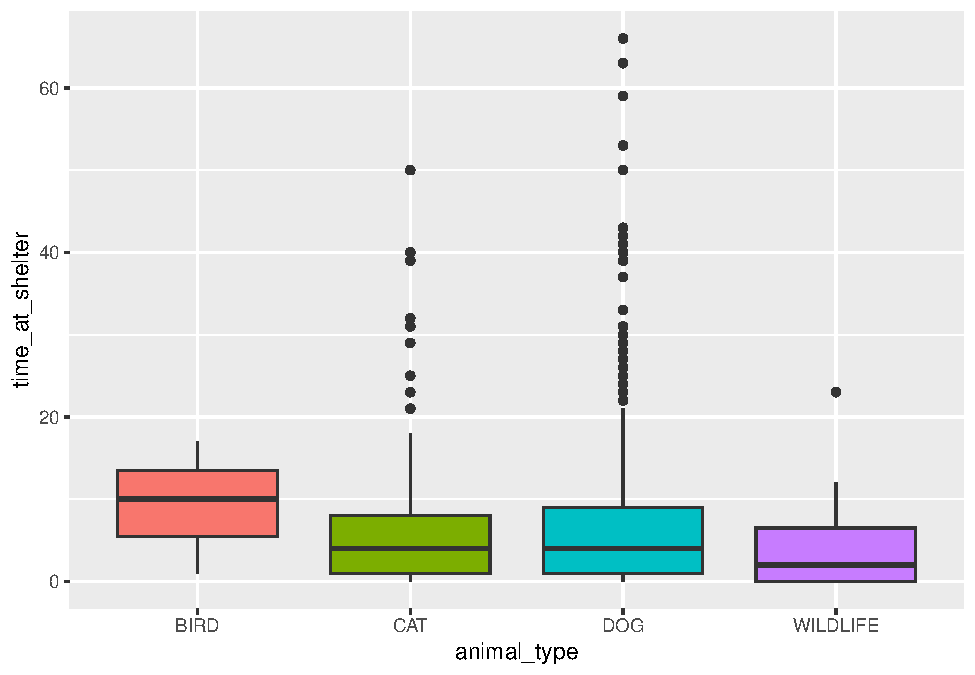
\includegraphics{Group_16_Project_version1_files/figure-latex/unnamed-chunk-2-1.pdf}

\begin{Shaded}
\begin{Highlighting}[]
\CommentTok{\#Plot of year against outcome\_type}
\FunctionTok{ggplot}\NormalTok{(}\AttributeTok{data =}\NormalTok{ df, }\FunctionTok{aes}\NormalTok{(}\AttributeTok{x =}\NormalTok{ year, }\AttributeTok{y =}\NormalTok{ time\_at\_shelter, }\AttributeTok{fill =}\NormalTok{ year)) }\SpecialCharTok{+}
  \FunctionTok{geom\_boxplot}\NormalTok{() }\SpecialCharTok{+}
  \FunctionTok{labs}\NormalTok{(}\AttributeTok{x =} \StringTok{"year"}\NormalTok{, }\AttributeTok{y =} \StringTok{"time\_at\_shelter"}\NormalTok{) }\SpecialCharTok{+}
  \FunctionTok{theme}\NormalTok{(}\AttributeTok{legend.position =} \StringTok{"none"}\NormalTok{)}
\end{Highlighting}
\end{Shaded}

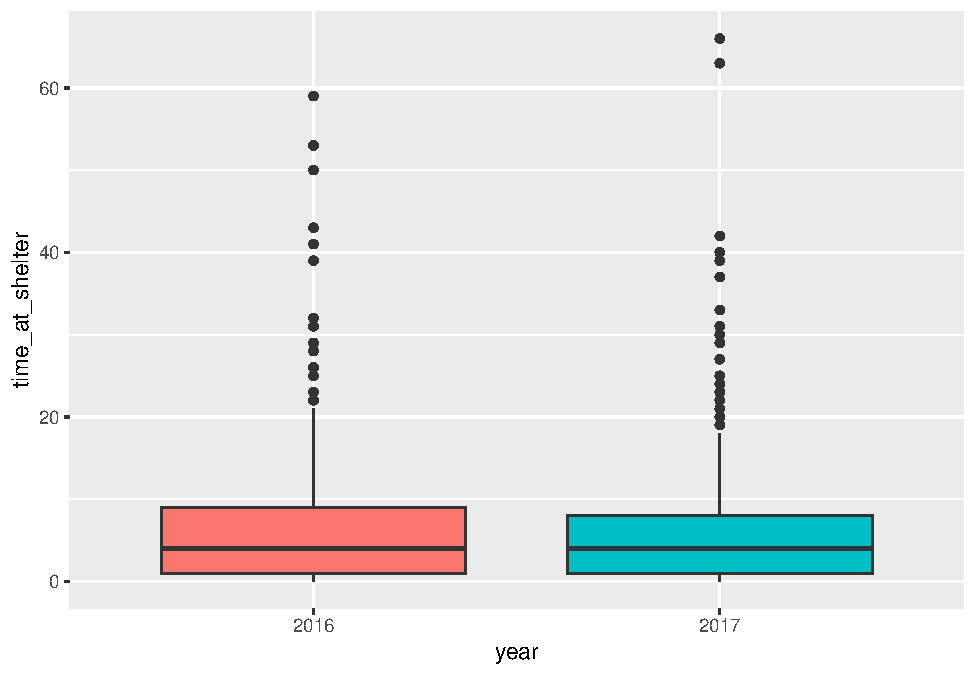
\includegraphics{Group_16_Project_version1_files/figure-latex/unnamed-chunk-3-1.pdf}

\begin{Shaded}
\begin{Highlighting}[]
\CommentTok{\#Plot of month against time\_at\_shelter}
\FunctionTok{ggplot}\NormalTok{(}\AttributeTok{data =}\NormalTok{ df, }\FunctionTok{aes}\NormalTok{(}\AttributeTok{x =}\NormalTok{ month, }\AttributeTok{y =}\NormalTok{ time\_at\_shelter, }\AttributeTok{fill =}\NormalTok{ month)) }\SpecialCharTok{+}
  \FunctionTok{geom\_boxplot}\NormalTok{() }\SpecialCharTok{+}
  \FunctionTok{labs}\NormalTok{(}\AttributeTok{x =} \StringTok{"month"}\NormalTok{, }\AttributeTok{y =} \StringTok{"time\_at\_shelter"}\NormalTok{) }\SpecialCharTok{+}
  \FunctionTok{theme}\NormalTok{(}\AttributeTok{legend.position =} \StringTok{"none"}\NormalTok{)}
\end{Highlighting}
\end{Shaded}

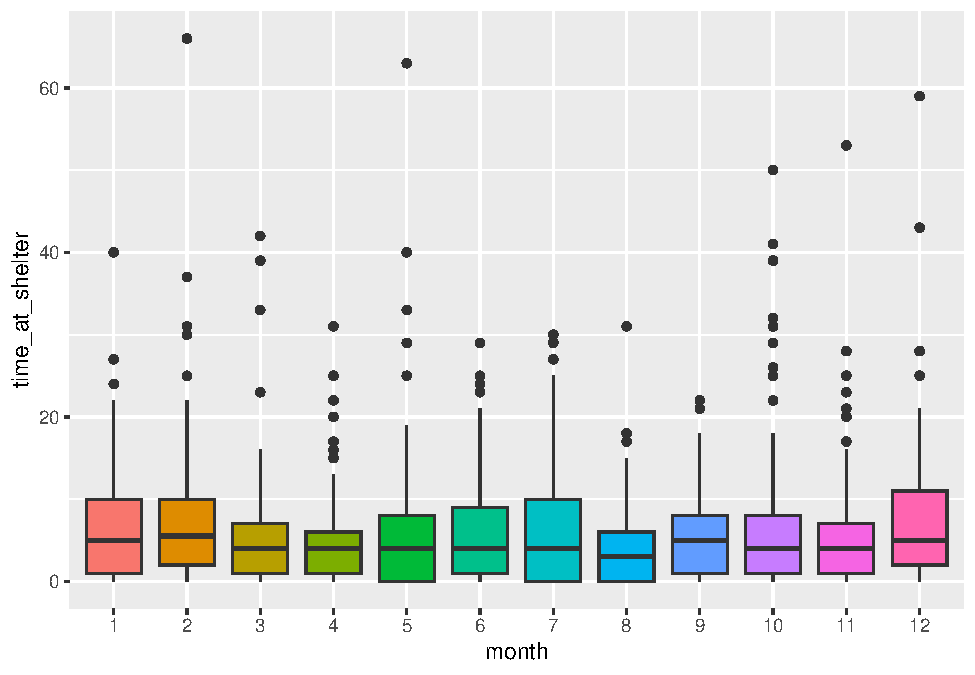
\includegraphics{Group_16_Project_version1_files/figure-latex/unnamed-chunk-4-1.pdf}

\begin{Shaded}
\begin{Highlighting}[]
\CommentTok{\#Plot of intake\_type against time\_at\_shelter}
\FunctionTok{ggplot}\NormalTok{(}\AttributeTok{data =}\NormalTok{ df, }\FunctionTok{aes}\NormalTok{(}\AttributeTok{x =}\NormalTok{ intake\_type, }\AttributeTok{y =}\NormalTok{ time\_at\_shelter, }\AttributeTok{fill =}\NormalTok{ intake\_type)) }\SpecialCharTok{+}
  \FunctionTok{geom\_boxplot}\NormalTok{() }\SpecialCharTok{+}
  \FunctionTok{labs}\NormalTok{(}\AttributeTok{x =} \StringTok{"intake\_type"}\NormalTok{, }\AttributeTok{y =} \StringTok{"time\_at\_shelter"}\NormalTok{) }\SpecialCharTok{+}
  \FunctionTok{theme}\NormalTok{(}\AttributeTok{legend.position =} \StringTok{"none"}\NormalTok{)}
\end{Highlighting}
\end{Shaded}

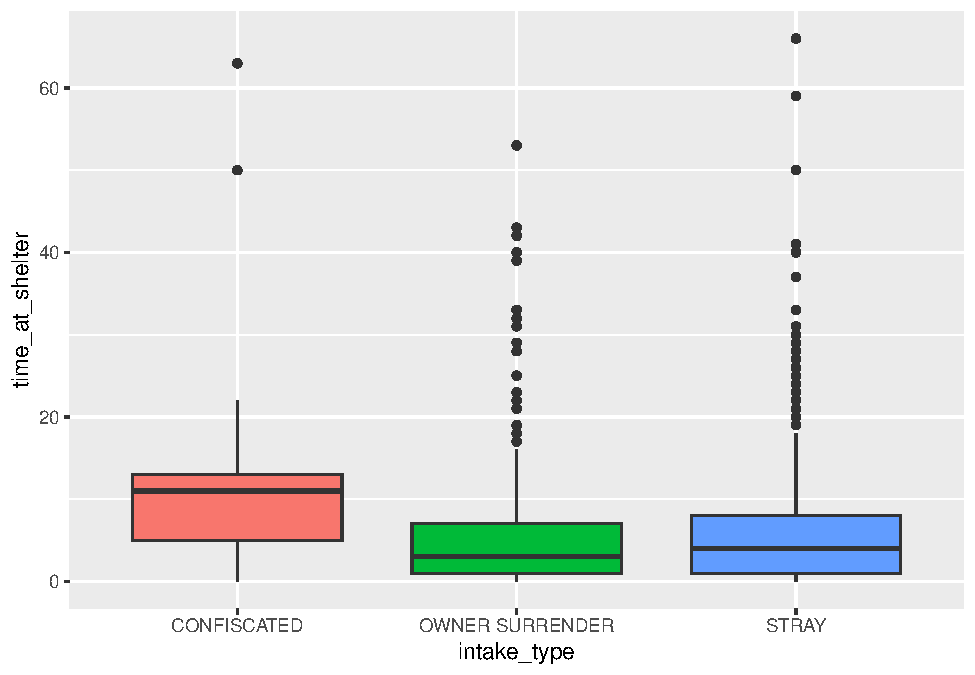
\includegraphics{Group_16_Project_version1_files/figure-latex/unnamed-chunk-5-1.pdf}

\begin{Shaded}
\begin{Highlighting}[]
\CommentTok{\#Plot of chip\_status against time\_at\_shelter}
\FunctionTok{ggplot}\NormalTok{(}\AttributeTok{data =}\NormalTok{ df, }\FunctionTok{aes}\NormalTok{(}\AttributeTok{x =}\NormalTok{ chip\_status, }\AttributeTok{y =}\NormalTok{ time\_at\_shelter, }\AttributeTok{fill =}\NormalTok{ chip\_status)) }\SpecialCharTok{+}
  \FunctionTok{geom\_boxplot}\NormalTok{() }\SpecialCharTok{+}
  \FunctionTok{labs}\NormalTok{(}\AttributeTok{x =} \StringTok{"chip\_status"}\NormalTok{, }\AttributeTok{y =} \StringTok{"time\_at\_shelter"}\NormalTok{) }\SpecialCharTok{+}
  \FunctionTok{theme}\NormalTok{(}\AttributeTok{legend.position =} \StringTok{"none"}\NormalTok{)}
\end{Highlighting}
\end{Shaded}

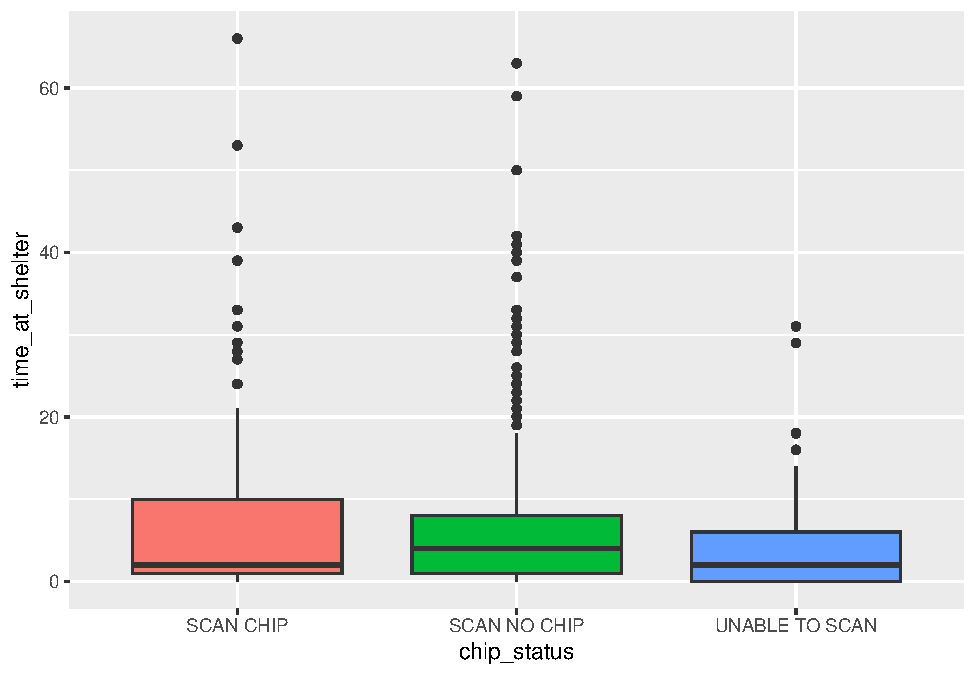
\includegraphics{Group_16_Project_version1_files/figure-latex/unnamed-chunk-6-1.pdf}

\begin{Shaded}
\begin{Highlighting}[]
\CommentTok{\#Modelling}
\NormalTok{model }\OtherTok{=} \FunctionTok{glm}\NormalTok{(time\_at\_shelter }\SpecialCharTok{\textasciitilde{}}\NormalTok{ animal\_type }\SpecialCharTok{+}\NormalTok{ month }\SpecialCharTok{+}\NormalTok{ year }\SpecialCharTok{+}\NormalTok{ intake\_type }\SpecialCharTok{+}\NormalTok{ chip\_status, }\AttributeTok{family=}\StringTok{"poisson"}\NormalTok{, }\AttributeTok{data=}\NormalTok{df)}
\CommentTok{\#Optimize the model}
\CommentTok{\#Summarize the first model}
\NormalTok{model }\SpecialCharTok{\%\textgreater{}\%}
  \FunctionTok{summary}\NormalTok{()}
\end{Highlighting}
\end{Shaded}

\begin{verbatim}

Call:
glm(formula = time_at_shelter ~ animal_type + month + year + 
    intake_type + chip_status, family = "poisson", data = df)

Deviance Residuals: 
    Min       1Q   Median       3Q      Max  
-4.9857  -2.6038  -0.7551   0.8060  12.7653  

Coefficients: (1 not defined because of singularities)
                           Estimate Std. Error z value Pr(>|z|)    
(Intercept)                 2.75306    0.19690  13.982  < 2e-16 ***
animal_typeCAT             -0.18315    0.19396  -0.944 0.345017    
animal_typeDOG             -0.23305    0.19251  -1.211 0.226055    
animal_typeWILDLIFE        -0.38615    0.22984  -1.680 0.092945 .  
month2                      0.14546    0.05533   2.629 0.008562 ** 
month3                     -0.25477    0.05692  -4.476 7.61e-06 ***
month4                     -0.28620    0.05657  -5.059 4.21e-07 ***
month5                     -0.11780    0.05181  -2.273 0.022996 *  
month6                     -0.08372    0.04991  -1.677 0.093482 .  
month7                     -0.14828    0.05051  -2.936 0.003327 ** 
month8                     -0.50955    0.05871  -8.679  < 2e-16 ***
month9                     -0.20499    0.05596  -3.663 0.000249 ***
month10                     0.05627    0.05167   1.089 0.276127    
month11                    -0.05734    0.05436  -1.055 0.291483    
month12                     0.16794    0.05157   3.257 0.001127 ** 
year2017                         NA         NA      NA       NA    
intake_typeOWNER SURRENDER -0.77494    0.04076 -19.012  < 2e-16 ***
intake_typeSTRAY           -0.58951    0.03765 -15.658  < 2e-16 ***
chip_statusSCAN NO CHIP    -0.01469    0.02805  -0.524 0.600525    
chip_statusUNABLE TO SCAN  -0.27589    0.06781  -4.068 4.73e-05 ***
---
Signif. codes:  0 '***' 0.001 '**' 0.01 '*' 0.05 '.' 0.1 ' ' 1

(Dispersion parameter for poisson family taken to be 1)

    Null deviance: 10551.2  on 1449  degrees of freedom
Residual deviance:  9957.4  on 1431  degrees of freedom
AIC: 14017

Number of Fisher Scoring iterations: 6
\end{verbatim}

\begin{Shaded}
\begin{Highlighting}[]
\CommentTok{\#Raise the second model by the summary table}
\CommentTok{\#Drop the year factor since it is only none value}
\NormalTok{model2 }\OtherTok{=} \FunctionTok{glm}\NormalTok{(time\_at\_shelter }\SpecialCharTok{\textasciitilde{}}\NormalTok{ animal\_type }\SpecialCharTok{+}\NormalTok{ month }\SpecialCharTok{+}\NormalTok{ intake\_type }\SpecialCharTok{+}\NormalTok{ chip\_status, }\AttributeTok{family=}\StringTok{"poisson"}\NormalTok{, }\AttributeTok{data=}\NormalTok{df)}
\CommentTok{\#Summarize the second model}
\NormalTok{model2 }\SpecialCharTok{\%\textgreater{}\%}
  \FunctionTok{summary}\NormalTok{()}
\end{Highlighting}
\end{Shaded}

\begin{verbatim}

Call:
glm(formula = time_at_shelter ~ animal_type + month + intake_type + 
    chip_status, family = "poisson", data = df)

Deviance Residuals: 
    Min       1Q   Median       3Q      Max  
-4.9857  -2.6038  -0.7551   0.8060  12.7653  

Coefficients:
                           Estimate Std. Error z value Pr(>|z|)    
(Intercept)                 2.75306    0.19690  13.982  < 2e-16 ***
animal_typeCAT             -0.18315    0.19396  -0.944 0.345017    
animal_typeDOG             -0.23305    0.19251  -1.211 0.226055    
animal_typeWILDLIFE        -0.38615    0.22984  -1.680 0.092945 .  
month2                      0.14546    0.05533   2.629 0.008562 ** 
month3                     -0.25477    0.05692  -4.476 7.61e-06 ***
month4                     -0.28620    0.05657  -5.059 4.21e-07 ***
month5                     -0.11780    0.05181  -2.273 0.022996 *  
month6                     -0.08372    0.04991  -1.677 0.093482 .  
month7                     -0.14828    0.05051  -2.936 0.003327 ** 
month8                     -0.50955    0.05871  -8.679  < 2e-16 ***
month9                     -0.20499    0.05596  -3.663 0.000249 ***
month10                     0.05627    0.05167   1.089 0.276127    
month11                    -0.05734    0.05436  -1.055 0.291483    
month12                     0.16794    0.05157   3.257 0.001127 ** 
intake_typeOWNER SURRENDER -0.77494    0.04076 -19.012  < 2e-16 ***
intake_typeSTRAY           -0.58951    0.03765 -15.658  < 2e-16 ***
chip_statusSCAN NO CHIP    -0.01469    0.02805  -0.524 0.600525    
chip_statusUNABLE TO SCAN  -0.27589    0.06781  -4.068 4.73e-05 ***
---
Signif. codes:  0 '***' 0.001 '**' 0.01 '*' 0.05 '.' 0.1 ' ' 1

(Dispersion parameter for poisson family taken to be 1)

    Null deviance: 10551.2  on 1449  degrees of freedom
Residual deviance:  9957.4  on 1431  degrees of freedom
AIC: 14017

Number of Fisher Scoring iterations: 6
\end{verbatim}

\end{document}
